\chapter{Relazione sui compiti svolti}
\label{cap:relazione}

\section{Strutturazione delle attività}
In questo capitolo verranno descritte in modo dettagliato tutte le varie
attività svolte presso la Wonderflow. Ogni sezione raggruppa le mansioni seguite
per realizzare uno specifico prodotto, in modo da esporre in maniera esaustiva
tutte le scelte, gli sviluppi ed i meccanismi messi in atto per portare a
termine il compito.

È da specificare che questo è frutto di un lavoro a posteriori: le varie azioni
conseguite furono pianificate senza una coesione logica e con una certa
discontinuità temporale. Solo a fine esperienza è stato possibile dedurre il
quadro d'insieme, impossibilitando però la produzione di una pianificazione che
seguisse il prodotto dall'inizio alla fine. Anche le stesse mansioni non hanno
sempre potuto godere di una progettazione allegata per via dello scarso
interesse che l'azienda nutre.

\section{Modulo NER}
\subsection{Esportatore annotazioni dalle recensioni}
\subsubsection{Requisiti}
Il funzionamento del modulo NER è strettamente legato al glossario di dove
pesca le annotazioni. Inizialmente il glossario è vuoto quindi i primi risultati
riporteranno la completa assenza di supporto da parte del modulo, ma man mano
che vengano aggiunte nuove annotazioni il sistema d'individuazione inizierà a
svolgere il suo compito. Tuttavia la qualità del servizio nei primi periodi
risentirà della scarsità d'annotazioni raccolte, impedendo di ottenere
suggerimenti che siano un'aiuto concreto all'analista.

Per evitare le basse \textit{performance} iniziali, la Wonderflow ha composto
un insieme di recensioni dove erano presenti annotazioni attentamente
controllate dai \textbf{Senior Analyst} la quale potevano offrire una buona base
di partenza per il glossario.

Il fatto delle annotazioni salvate come attributo della recensione d'origine
però poneva grossi problemi. In primo luogo, ogni programma che gestiva solo
annotazioni avrebbe dovuto conoscere lo schema delle recensioni, creando un
accoppiamento indesiderato; secondo, la semplicità di gestione ed uso
dell'archivio verrebbe meno, principalmente per il fatto di non avere una
relazione \textit{uno a molti} tra annotazione e recensioni.

Necessariamente progettare uno schema che ponesse l'accento sulle annotazioni
piuttosto che sulle recensioni diventava indispensabile. Altro elemento
fondamentale era compiere l'estrazione e la conversione delle annotazioni al
nuovo formato progettato.

Queste due richieste sono state tradotte nella creazione di:
\begin{itemize}
\item Un \gls{DAO} per gestire oggetti \textit{MongoDB} conformi al nuovo schema
dell'annotazione
\item Script \textit{Node.js} che esporta, modifica e salva le annotazione dal
vecchio al nuovo formato
\end{itemize}

La realizzazione di un \gls{DAO} segue sia una norma interna, dove ogni
entità di natura persistente all'interno della compagnia richiede la
realizzazione di un archivio e di un \gls{DAO} associato, sia la sua effettiva
praticità d'uso.

\subsubsection{Sviluppo}
Data la dipendenza dello script con il modulo \gls{DAO} associato alle nuove
annotazioni è stato considerato valido partire con lo sviluppo di quest'ultimo.

La Wonderflow raggruppa i propri \gls{DAO} in un pacchetto \textit{npm} chiamato
``\textit{models}'' in modo che, ogni qualvolta è richiesto l'accesso al
database, sia sufficiente includerlo nel proprio progetto e importare il
\gls{DAO} desiderato. La parte relativa al progetto è illustrata in figura
\ref{fig:dao_annotation}.

\begin{figure}[H]
\begin{center}
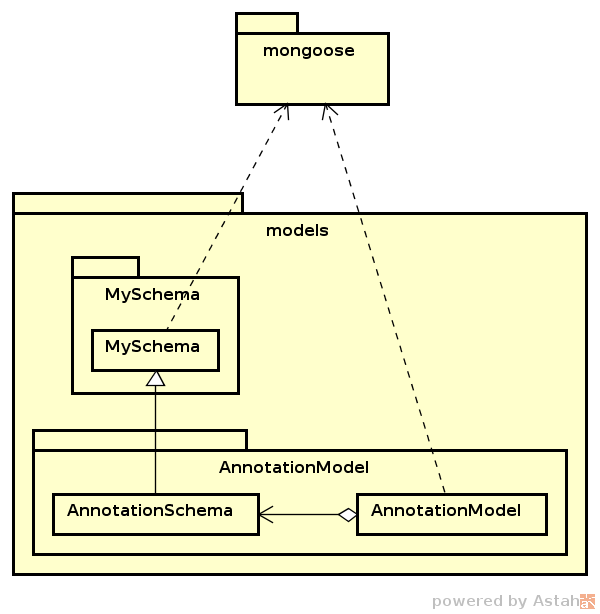
\includegraphics[height=9cm]{dao_annotation}
\caption{
Rappresentazione DAO per le annotazioni nel pacchetto ``\textit{models}''
}
\label{fig:dao_annotation}
\end{center}
\end{figure}

Il package \textit{mongoose} rappresenta il pacchetto \textit{npm} con il quale
vengono implementati i \gls{DAO}. Vi sono due elementi elementi in
\textit{mongoose}: lo \textbf{schema} ed il \textbf{modello}.

Il primo è ciò che rende questo pacchetto molto versatile alla modellazione dei
dati di un'applicazione. Attraverso la definizione di un oggetto in JavaScript è
possibile definire di quali \textbf{attributi} il dato da modellare è composto e
quali metodi il \gls{DAO} ha per interfacciarsi con esso. Nel caso in specie
``\textit{AnnotationSchema}'' definisce come ``annotazione'' un oggetto conforme
al seguente schema:
\begin{center}
\begin{lstlisting}[
  frame=single,
  caption=Schema entità 'annotazione',
  label=valid_annotation]
{
    "uid": "String",
    "name": "String",
    "text": "String",
    "syn": "String",
    "sentiment": 0 | 1,
    "category": "String",
    "reviews": [{
       "id": "String",
       "start": "Number",
       "offset": "Number",
       "origin": "pros" | "cons" | "free-text",
       "version": "String"
    }]
}
\end{lstlisting}
\end{center}

mentre il \gls{DAO} eredita i metodi \textit{CRUD (create, read, update,
delete)}\footnote{Per una maggior trattazione si veda
\url{http://coursework.vschool.io/mongoose-crud/}}, implementati dal
``\textit{model}'' base di \textit{mongoose}, ed il metodo per effettuare la
connessione al database da ``\textit{MySchema}''. Inoltre aggiunge un
ulteriore metodo di classe: ``\textit{insertOrMerge}''.

La descrizione del metodo verrà approfondita in seguito.

Come si può notare il nuovo schema dell'annotazione è molto simile a quello
risultante dal processo d'analisi, discusso nella sezione
\ref{subsec:processo_recensioni_annotazioni}, ma vi sono alcune differenze che
risolvono egregiamente tutte le problematiche riscontrate:
\begin{itemize}
\item L'annotazione non è più un attributo ma copre il ruolo d'oggetto unico
\item I riferimenti alla recensione in cui appare l'annotazione vengono salvati
nel campo ``\textit{reviews}''
\end{itemize}

Con la prima modifica si rimuove l'accoppiamento indesiderato con la recensione.
Ora un qualsiasi programma che avesse esclusivamente bisogno delle annotazioni
non è vincolato a conoscere la struttura delle recensioni.

Con la seconda modifica invece gira la relazione \textit{uno a molti} tra
la recensione e l'annotazione, ottenendo che nell'annotazione si mantengono i
riferimenti alle recensioni in cui appare. La gestione dei riferimenti è
compito del \textit{insertOrMerge} citato sopra. La sua funzione è di o inserire
la nuova annotazione se non è già presente o di agganciare i riferimenti alle
recensioni non ancora presenti nell'attributo ``\textit{reviews}'', mantenendo
cosi la relazione desiderata.

L'ultimo aspetto da chiarire è il \textbf{modello} di \textit{mongoose},
implementato dalla classe ``AnnotationModel''. Il modello, attraverso lo schema,
funge da costruttore per oggetti legati ad un documento \textit{MongoDB} e
provvisti di tutti i metodi per interfacciarsi. In breve, il modello è il
costruttore dei \gls{DAO}. Nel caso di ``AnnotationModel'' i \gls{DAO}
costruiti sono inerenti alle annotazioni e legati al documento
``\textit{Annotation}''. \\

Una volta completata la parte per accedere e manipolare documenti relativi
alla nuova struttura dell'annotazione, si è prodotto lo \gls{script} per
estrarre le annotazioni già presenti nell'archivio aziendale. Il riassunto del
processo è illustrato in figura \ref{fig:extractor_annotation}.

\begin{figure}[H]
\begin{center}
\includegraphics[height=6cm]{extractor_annotation}
\caption{
Rappresentazione processo d'estrazione e trasformazione delle annotazioni
}
\label{fig:extractor_annotation}
\end{center}
\end{figure}

Lo script è organizzato sottoforma di \gls{pipeline} sfruttando l'interfaccia
``\textit{stream}'' di \textit{Node.js} e la libreria \textit{through2}. La
\gls{pipeline} è composta da tre elementi:
\begin{itemize}
\item ReaderData - legge le recensioni dentro l'archivio e crea lo
\textit{stream}
\item AnnotationExtractor - estrae e applica le debite trasformazioni alle
annotazioni
\item AnnotationWriter - scrive le annotazioni nell'archivio
\end{itemize}

Il ``ReaderData'' usa il \gls{DAO} apposito per le recensioni per leggerle tutte
e generare uno ``\textit{stream}'' con il quale le invierà, di volta in volta,
all'``AnnotationExtractor'' tramite il metodo \textit{.pipe()}.

Il metodo permette la comunicazione tra le unità consecutive della
\textit{pipeline} attraverso la generazione d'eventi il cui contenuto
trasportato è il risultato dell'unita precedente. Nel caso tra ``ReaderData'' e
``AnnotationExtractor'' il contenuto è la recensione estratta, mentre tra
``AnnotrationExtractor'' e ``AnnotationWriter'' è l'annotazione modificata
conforme allo schema \ref{valid_annotation}.

Quando ``AnnotationExtractor'' riceve la recensione applica l'algoritmo di
trasformazione illustrato nel diagramma d'attività
\ref{fig:extractor_annotation}. La recensione in input immagazzina le
annotazioni nell'attributo ``\textit{feature2sentiment}''. Tutte le recensioni
con la versione diversa da ``v2'' vengono immediatamente scartate, in modo da
non complicare l'algoritmo d'estrazione. Il corpo centrale del diagramma ha lo
scopo di ribaltare la relazione tra recensione ed annotazione. Gli attributi:
\textit{version, start, offset e origin} sono dipendenti dalla recensione in
cui l'annotazione era stata individuata; perciò vengono inglobati in un unico
oggetto, identificato con l'id della recensione e inserito nell'annotazione
nell'attributo ``\textit{reviews}''. Una volta terminate tutte le annotazioni,
il risultato finale viene trasmetto all'unità successiva.

\begin{figure}[H]
\begin{center}
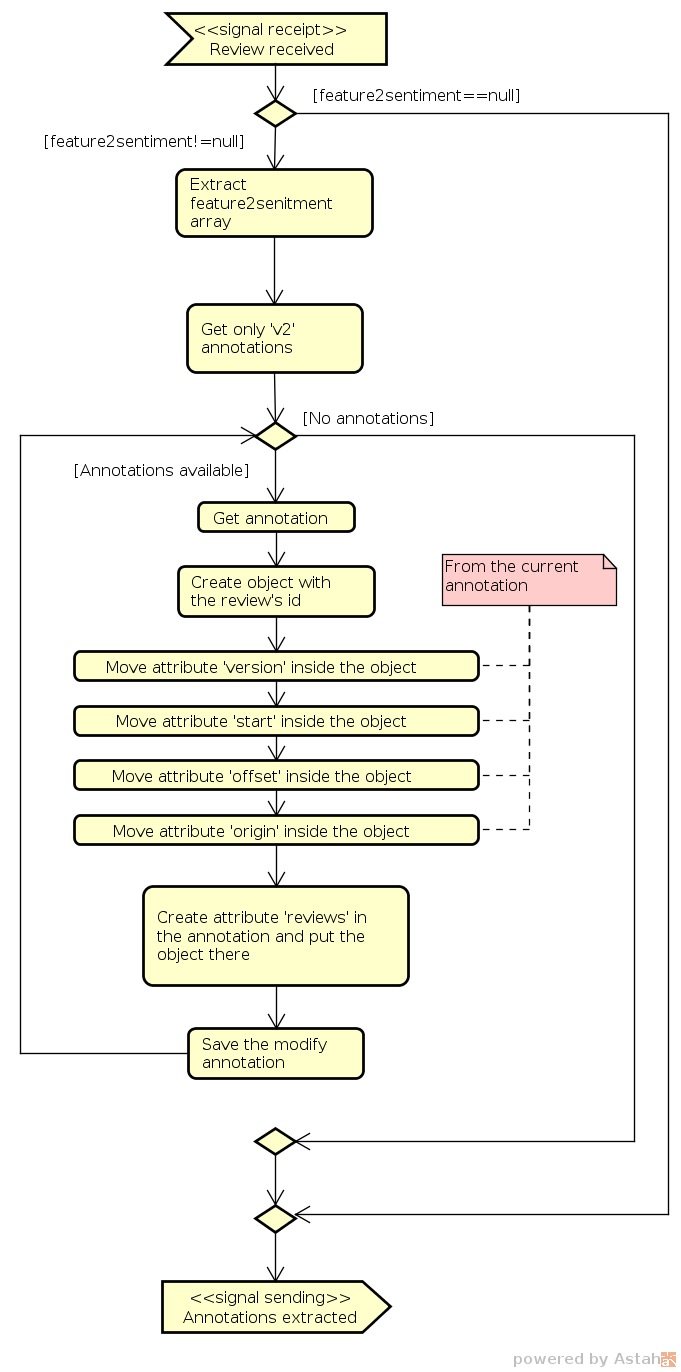
\includegraphics[height=15cm]{extraction_activity}
\caption{
Diagramma d'attività trasformazione annotazioni
}
\label{fig:extraction_activity}
\end{center}
\end{figure}

``AnnotationWriter'' per salvare le annotazioni ricevute nel database, invoca il
metodo \textit{.insertOrMerge()} del \gls{DAO} creato nella fase precedente. In
tal modo, l'unità di scrittura, non dovrà preoccuparsi di come venga mantenuta
la relazione tra annotazioni e recensioni cosi da non violare il
\textit{Single Responsability Principle}.

\subsubsection{Test}
%
%\subsection{Applicazione Java per riconoscere le annotazioni}
%\subsubsection{Requisiti}
%\subsubsection{Sviluppo}
%\subsubsection{Test}
%
%\subsection{Integrazione con il tool esistente}
%\subsubsection{Requisiti}
%\subsubsection{Script d'integrazione}
%\subsubsection{Script di misurazione qualità}
%
%\section{Moderazione del glossario}
%\subsection{Comunicazione con il backend}
%\subsubsection{Funzionamento}
%\subsubsection{Modello dell'annotazione}
%\subsubsection{Ampliamento modello della recensione}
%
%\subsection{Interfaccia web}
%\subsubsection{Requisiti}
%\subsubsection{Sviluppo}
%\subsubsection{Test}
%
%\section{Refactoring del BaaS}
%\subsection{Stato iniziale}
%
%\subsection{Progettazione}
%
%\subsection{Ristrutturazione HTTP Handler}
%\subsubsection{Requisiti}
%\subsubsection{Funzionamento}
%\subsubsection{Test}
%
%\subsection{Ristrutturazione applicazione Express}
%\subsubsection{Requisiti}
%\subsubsection{Funzionamento}
%\subsubsection{Test}
%
%\subsection{Ristrutturazione Wonderflow API}
%\subsubsection{Requisiti}
%\subsubsection{Funzionamento}
%\subsubsection{Test}
%
%\subsection{Collaudo e pubblicazione}
%
%\section{Generatore Yeoman per applicazioni AngularJS}
%\subsection{Requisiti}
%\subsection{Funzionamento}
%\subsection{Test}
%
